\documentclass[11pt]{article}
\usepackage[UTF8]{ctex}
\usepackage[a4paper]{geometry}
\geometry{left=2.0cm,right=2.0cm,top=2.5cm,bottom=2.5cm}

\usepackage{comment}
\usepackage{booktabs}
\usepackage{graphicx}
\usepackage{diagbox}
\usepackage{amsmath,amsfonts,graphicx,amssymb,bm,amsthm,enumitem}
%\usepackage{algorithm,algorithmicx}
\usepackage[ruled]{algorithm2e}
\usepackage[noend]{algpseudocode}
\usepackage{fancyhdr}
\usepackage{tikz}
\usepackage{graphicx}
\usetikzlibrary{arrows,automata}
\usepackage{hyperref}
\hypersetup{
	colorlinks=true,
	linkcolor=blue,
	filecolor=blue,      
	urlcolor=blue,
	citecolor=cyan,
}			

\setlength{\headheight}{14pt}
\setlength{\parindent}{0 in}
\setlength{\parskip}{0.5 em}

\newtheorem{theorem}{Theorem}
\newtheorem{lemma}[theorem]{Lemma}
\newtheorem{proposition}[theorem]{Proposition}
\newtheorem{claim}[theorem]{Claim}
\newtheorem{corollary}[theorem]{Corollary}
\newtheorem{definition}[theorem]{Definition}
\newtheorem*{definition*}{Definition}

\newenvironment{problem}[2][Problem]{\begin{trivlist}
\item[\hskip \labelsep {\bfseries #1}\hskip \labelsep {\bfseries #2.}]}{\hfill$\blacktriangleleft$\end{trivlist}}
\newenvironment{answer}[1][Answer]{\begin{trivlist}
\item[\hskip \labelsep {\bfseries #1.}\hskip \labelsep]}{\hfill$\lhd$\end{trivlist}}

\newcommand\E{\mathbb{E}}
\newcommand\per{\mathrm{per}}


\title{Homework \#2}
\usetikzlibrary{positioning}

\begin{document}

\pagestyle{fancy}
\lhead{Peking University}
\chead{}
\rhead{Mathematical Foundations for the Information Age, 2025 Fall}

\begin{center}
    {\LARGE \bf Homework \#2}\\
    {Due: 2025-11-16 23:59 \quad$|$\quad 7 Problems, 100 Pts}\\
    {Name: 李思成, ID: 2400017787}            % Write down your name and ID here.
\end{center}



\begin{problem}{1 (20')} Consider a cube $C$ with side length $1$ in $d$-dimensional space.
\begin{itemize}
    \item [(1)] (4') Write down the radius of a ball $B$ whose volume is equal to the cube's. You don't need to prove your result.
    \item [(2)] (16') When the centers of the cube $C$ and the ball $B$ are both at the origin, calculate the volume of their intersection when $d\to+\infty$.
    \item [] \textit{[Hint: Try to calculate $\mathbb{E}_{X\sim C}[\|X\|_2^2]$ and $Var_{X\sim C}[\|X\|_2^2]$. Then use Chebyshev's Inequality to analyze the concentration of $\|X\|_2^2$. You may use the Stirling's approximation}
    \begin{align*}
        \lim_{n\to+\infty}\frac{\Gamma(n+1)}{\sqrt{2\pi n}(n/\mathrm{e})^n}=1.\tag*{\textit{]}}
    \end{align*}
\end{itemize}
\end{problem}

\begin{answer} ~
    \begin{itemize}
        \item[(1)] The radius is \[r = \frac{1}{\sqrt{\pi}}\left(\frac{d}{2}\Gamma\left(\frac{d}{2}\right)\right)^\frac{1}{d}\].
        \item[(2)] First, let $X \sim C$, $X = (x_1, \dots, x_d)$, then $x_i \sim U(-\frac{1}{2}, \frac{1}{2})$ and $x_i$ pairwise independent. We can calculate that
        \begin{align*}
            &\forall i, \E[x_i^2] = \int_{-\frac{1}{2}}^{\frac{1}{2}} x^2 dx = \frac{1}{12} \\
            &\Rightarrow \E[\|X\|^2] = \E\left[\sum_{i=1}^d x_i^2\right] = \frac{d}{12} \\
            &\forall i, \E[x_i^4] = \int_{-\frac{1}{2}}^{\frac{1}{2}} x^4 dx = \frac{1}{80} \\
            &\Rightarrow \E[\|X\|^4] = \sum_{i=1}^d \E[x_i^4] + 2\sum_{i\neq j} \E[x_i^2]\E[x_j^2] = \frac{d}{80} + 2\binom{d}{2} \frac{1}{12} \frac{1}{12} = \frac{d^2}{144} + \frac{d}{180} \\
            &\Rightarrow Var[\|X\|^2] = \E[\|X\|^4] - (\E[\|X\|^2])^2 = \frac{d}{180} 
        \end{align*}
        Then, use Stirling's Formula, 
        \begin{align*}
            \frac{r^2}{\frac{d}{12}} &\sim \frac{12}{\pi d} \left(\sqrt{\pi d}\left(\frac{d}{2\mathrm{e}}\right)^{\frac{d}{2}}\right)^\frac{2}{d} \\
            &= \frac{12}{\pi d} (\sqrt{\pi d})^\frac{2}{d} \left(\frac{d}{2\mathrm{e}}\right) \\
            &\to \frac{6}{\mathrm{e}\pi} < 1, d \to \infty
        \end{align*}
        This implies $r^2 < \frac{d}{12}$ when $d$ is large enough. As a result, with Chebyshev's Inequality,
        \begin{align*}
            \frac{V(B \cap C)}{V(C)} &= \Pr_{X \sim C}[X \in B] \\
            &= \Pr_{X \sim C}\left[\|X\|^2 \leq r^2\right] \\
            &= \Pr_{X \sim C}\left[\|X\|^2 - \E[\|X\|^2] \le r^2 - \frac{d}{12}\right] \\
            &= \Pr_{X \sim C}\left[\|X\|^2 - \E[\|X\|^2] \le -\left|r^2 - \frac{d}{12}\right|\right] \\
            &\le \Pr_{X \sim C}\left[\left|\|X\|^2 - \E[\|X\|^2]\right| \ge \left|r^2 - \frac{d}{12}\right|\right] \\
            &\le \frac{Var[\|X\|^2]}{\left(r^2 - \frac{d}{12}\right)^2} \\
            &= \frac{1}{180} \frac{d}{\left(r^2 - \frac{d}{12}\right)^2} \\
            &= \frac{1}{180} \frac{d}{\left(\left(\frac{6}{\mathrm{e}{\pi}} - 1 + o(1)\right)\frac{d}{12}\right)^2} \\
            &= O\left(\frac{1}{d}\right) \to 0, d \to \infty
        \end{align*}
        Since $V(C) = 1$, $V(B \cap C) \to 0$ as $d \to \infty$.
    \end{itemize}
\end{answer}

\begin{problem}{2 (16')}
You select a PE class this term, so you need to complete a total of 85km of extracurricular exercise. There are only $n$ days before the deadline, but you still have $m$ kilometers remaining. To simplify your work, you can run at most 10km every day, but there is no lower bound. You are mindless when running, so the distance you run every day is uniformly random. In other words, the number of kilometers you run every day is a real number uniformly selected from range $[0,10]$. Prove that, the probability that you can complete $m$ kilometers in $n$ days, i.e., the probability that your total distance in $n$ days is greater than or equal to $m$ kilometers is 
\begin{align*}
    1-\sum_{i=0}^{\min(\lfloor m/10\rfloor,n)}\frac{(-1)^i}{i!(n-i)!}\left(\frac{m}{10}-i\right)^n.
\end{align*}
\end{problem}

\begin{answer} ~

    Let 
    \[C = \{(x_1, \dots, x_n) \in \mathbb{R}^n \ | \ \forall i, 0 \le x_i \le 10\}\]
    \[T = \{(x_1, \dots, x_n) \in \mathbb{R}^n \ | \ \forall i, x_i \ge 0; \sum_{i=1}^n x_i \le m\}\]
    In Homework \#1, we have calculated that $V(T) = m^n/n!$. If we randomly pick $X = (x_1, \dots, x_n)$ in $T$, then
    \begin{align*}
        1 - \frac{V(C \cap T)}{V(T)} &= \Pr_{X \sim T}[\exists i, x_i > 10] \\
        &= \Pr_{X \sim T}\left[\bigcup_{i=1}^n A_i \right] (A_i := ``x_i > 10") \\
        &= \sum_{i=1}^n \sum_{j_1 < \dots < j_i} (-1)^{i-1} \Pr_{X \sim T}\left[A_{j_1} \cap \dots \cap A_{j_i} \right] \\
        &= \sum_{i=1}^n (-1)^{i-1} \binom{n}{i} \Pr_{X \sim T} [A_1 \cap \dots \cap A_i] \\
        &= \sum_{i=1}^n (-1)^{i-1} \binom{n}{i} \Pr_{X \sim T} [x_1 > 10, \dots, x_i > 10] \\
        &= \sum_{i=1}^n (-1)^{i-1} \binom{n}{i} V\left(\left\{X' \in \mathbb{R}^n \ | \ \forall j, x_j' \ge 0, \sum_{j=1}^n x_j' \le m - 10i \right\}\right) / V(T) \\
        &= \sum_{i=1}^{\min(n, \lfloor m/10 \rfloor)} (-1)^{i-1} \binom{n}{i} \left(1 - \frac{10}{m}i\right)^n
    \end{align*}
    Hence
    \begin{align*}
        V(C \cap T) = 10^n \sum_{i=0}^{\min(n, \lfloor m/10 \rfloor)} \frac{(-1)^{i}}{i!(n-i)!} \left(\frac{m}{10} - i\right)^n
    \end{align*}
    The probability that we want to calculate is $Pr_{X \sim C}[X \notin T]$, so the final answer is
    \[1 - \frac{V(C \cap T)}{V(C)} = 1 - \sum_{i=0}^{\min(n, \lfloor m/10 \rfloor)} \frac{(-1)^{i}}{i!(n-i)!} \left(\frac{m}{10} - i\right)^n\]
    
\end{answer}

\begin{problem}{3 (10')}
If $A$ is square, show that $AA^\top$ and $A^\top A$ are similar.

\textit{[Hint: Use the SVD of $A$.]}
\end{problem}

\begin{answer} ~

    According to SVD, there exists two orthogonal matrices $U, V$ and a diagonal matrix $\Sigma$ such that $A = U\Sigma V^\top$. Then
    \[AA^\top = U\Sigma V^\top V\Sigma U^\top = U\Sigma^2U^\top\]
    \[A^\top A = V\Sigma U^\top U \Sigma V^\top = V\Sigma^2 V^\top\]
    So $AA^\top$ and $A^\top A$ are both similar to $\Sigma^2$.
    
\end{answer}

\begin{problem}{4 (12')}
Calculate the SVD of matrix $A$, where 
\begin{align*}
    A=\begin{pmatrix}
        -4&-6\\3&-8
    \end{pmatrix}.
\end{align*} 
You need to calculate it in two different ways.

\textit{[Hint: Use the definition of singular vectors, or consider $A^\top A$.]}
\end{problem}

\begin{answer} ~

    First, we use the definition of singular values. Set $v = \begin{pmatrix} x_1 \\ x_2 \end{pmatrix}$ where $x_1^2 + x_2^2 = 1$, then
    \[Av = \begin{pmatrix} -4 & -6 \\ 3 & -8 \end{pmatrix} \begin{pmatrix} x_1 \\ x_2 \end{pmatrix} = \begin{pmatrix} -4x_1 -6x_2 \\ 3x_1 - 8x_2 \end{pmatrix}\]
    \[\|Av\|^2 = 25x_1^2 + 100x_2^2 = 25 + 75x_2^2\]
    To maximize $\|Av\|^2$，let $x_2 = 1$, $x_1 = 0$, then the first singular vector $v_1 = (0, 1)^\top$, and the first singular value $\sigma_1 = 10$. Let $v \perp v_1$, then $v$ can only be $(\pm 1, 0)^\top$, thus we take the second singular vector $v_2 = (1, 0)^\top$ and the second singular value $\sigma_2 = 5$. As a result,
    \[A = \begin{pmatrix} -0.6 & -0.8 \\ -0.8 & 0.6 \end{pmatrix} \begin{pmatrix} 10 & 0 \\ 0 & 5 \end{pmatrix} \begin{pmatrix} 0 & 1 \\ 1 & 0 \end{pmatrix}\]

    Second, we perform diagonalization on $A^\top A$. 
    \[A^\top A = \begin{pmatrix} 25 & 0 \\ 0 & 100 \end{pmatrix}\]
    So its eigenvalues are $\lambda_1 = 100$ and $\lambda_2 = 25$, thus the singular values of $A$ is $\sigma_1 = 10$ and $\sigma_2 = 5$. For $i = 1, 2$ solve the equation $\det(\lambda_i I - A^\top A)v = 0$, we get two eigenvectors $v_1 = (0, 1)^\top$ and $v_2 = (1, 0)^\top$. The final answer is the same as the first method.
    
\end{answer}

\begin{problem}{5 (16')}
Let $A=\sum_{i=1}^{r}\sigma_iu_iv_i^\top$ be the SVD of a rank-$r$ matrix $A$, let $A_k:=\sum_{i=1}^k\sigma_iu_iv_i^\top$ be the rank-$k$ approximation of $A$ for some $k<r$. 
\begin{itemize}
    \item [(1)] (4') Express the following quantities in terms of the singular values $\{\sigma_i,1\le i\le r\}$. You don't need to prove your result.
    \begin{itemize}
        \item [(a)] (2') $\|A_k\|_F^2$.
        \item [(b)] (2') $\|A_k\|_2^2$.
    \end{itemize}
    \item [(2)] (3') Prove that, $\sigma_k\le \frac{\|A\|_F}{\sqrt{k}}$ for $k=1,2,\cdots,r$.
    \item [(3)] (9') Suppose $A\in\mathbb{R}^{m\times m}$. Let $B=\sum_{i=1}^r\frac{1}{\sigma_i}v_iu_i^\top$.  
    \begin{itemize}
        \item [(a)] (6') Show that $BAx=x$ for all $x$ in the span of the right singular vectors of $A$. For this reason $B$ is sometimes called the pseudo inverse of $A$ and can play the role of $A^{-1}$ in many applications.
        \item [(b)] (3') Does $BAx=x$ always hold for all $x\in\mathbb{R}^m$? Prove or give a counterexample.
    \end{itemize}
\end{itemize}
\end{problem}

\begin{answer} ~
    \begin{itemize}
        \item[(1)]
        \begin{itemize}
            \item[(a)] $\|A_k\|_F^2 = \sigma_1^2 + \dots + \sigma_k^2$.
            \item[(b)] $\|A_k\|_2^2 = \sigma_1^2$.
        \end{itemize}
        \item[(2)] $\forall k = 1, 2, \dots, r$, 
            \[\|A\|_F^2 = \sigma_1^2 + \dots + \sigma_k^2 + \sigma_{k+1}^2 + \dots + \sigma_r^2 \ge \sigma_k^2 + \dots + \sigma_k^2 + 0 + \dots + 0 = k\sigma_k^2\]
            So $\sigma_k \le \frac{\|A\|_F}{\sqrt{k}}$.
        \item[(3)]
        \begin{itemize}
            \item[(a)] \[BA = \left(\sum_{i=1}^r \frac{1}{\sigma_i} v_i u_i^\top \right) \left(\sum_{i=1}^r \sigma_i u_i v_i^\top \right) = \sum_{i=1}^r v_i v_i^\top\]
            Then for any $v \in \langle v_1, \dots, v_r \rangle$, $v = \sum_{i=1}^r c_i v_i$, $BAv = \sum_{i=1}^r c_i v_i v_i^\top v_i = v$.
            \item[(b)] No. Choose any matrix $A$ that is not full rank, then $r < m$. There exists a vector $u \in \mathbb{R}^m, u \perp \langle v_1, \dots, v_r \rangle$ and $u \neq 0$, but $BAu = 0$.
        \end{itemize}
    \end{itemize}
\end{answer}

\begin{problem}{6 (16')}
In class, we introduced the best-fit subspace for a set of points. We extend this definition to probability densities instead of a set of points. If $P$ is a probability density in $\mathbb{R}^d$, then we define the best-fit $k$-dimensional subspace ($k\leq d$)
\begin{align*}
V_k=\arg\max_{V,\mathrm{dim}(V)=k}\E_{X\sim P}(|\mathrm{proj}(X,V)|^2),
\end{align*}
where $\mathrm{proj}(X,V)$ is the orthogonal projection of $X$ onto $V$.
\begin{itemize}
    \item [(1)] (6') Find out the best-fit $1$-dimensional subspace (i.e., a best-fit line through the origin) for probability density $\mathcal{N}\left(0,0,1,2,\frac{1}{2}\right)$.
    \item [] \textit{[Hint: Suppose random variable $(X_1,X_2)\sim\mathcal{N}\left(0,0,1,2,\frac{1}{2}\right)$, then we have}
    \begin{align*}
        X_1\sim\mathcal{N}(0,1),\;X_2\sim\mathcal{N}(0,2),\;\rho:=\frac{\mathbb{E}(X_1X_2)-\mathbb{E}(X_1)\mathbb{E}(X_2)}{\sqrt{Var(X_1)Var(X_2)}}=\frac12.\tag*{\textit{]}}
    \end{align*}
    \item [(2)] (10') Prove that, for $d$-dimensional Gaussian distribution $\mathcal{N}(\mu,I_d)$, a $k$-dimensional subspace is a best-fit subspace if and only if it contains $\mu$.
    \item [] \textit{[Hint: Suppose random variable $(X_1,\cdots,X_d)\sim\mathcal{N}(\mu,I_d)$, then we have $X_i\sim\mathcal{N}(\mu_i,1)$ and $X_1,\cdots,X_d$ are independent random variables.]}
\end{itemize}
\end{problem}

\begin{answer} ~
    \begin{itemize}
        \item[(1)] Let $X = (X_1, X_2)^\top \sim \mathcal{N}(0, 0, 1, 2, \frac{1}{2})$, then $X_1 \sim \mathcal{N}(0, 1)$, $X_2 \sim \mathcal{N}(0, 2)$, and $\rho = \frac{1}{2} \Rightarrow \E(X_1 X_2) = \frac{\sqrt{2}}{2}$. Assume $V$ is determined by a unit vector $v = (v_1, v_2)^\top$, then
        \[|\mathrm{proj}(X, V)|^2 = (X^\top v)^2 = v_1^2X_1^2 + v_2^2X_2^2 + 2v_1v_2X_1X_2\]
        \begin{align*}\E_{X\sim P}(|\mathrm{proj}(X, V)|^2) &= v_1^2 + 2v_2^2 + \sqrt{2}v_1v_2 \\ &\le v_1^2 + 2v_2^2 + \frac{(\sqrt{3} + 1)v_1^2 + (\sqrt{3} - 1)v_2^2}{2} \\ &= \frac{3 + \sqrt{3}}{2}\end{align*}
        Maximum is achieved iff $(\sqrt{3} + 1)v_1^2 = (\sqrt{3} - 1)v_2^2$, i.e. $v = \pm\left(\sqrt{\frac{3 - \sqrt{3}}{6}}, \sqrt{\frac{3 + \sqrt{3}}{6}}\right)^\top$,
        \[V_1 = \left\langle \left(\sqrt{\frac{3 - \sqrt{3}}{6}}, \sqrt{\frac{3 + \sqrt{3}}{6}}\right)^\top\right\rangle\]
        \item[(2)] Let $X = (X_1, \dots, X_d)^\top \sim \mathcal{N}(\mu, I_d)$, then $X_i \sim \mathcal{N}(\mu_i, 1)$ and $X_i$ independent. Pick an orthonormal basis $v_1, \dots, v_k \in V$, $v_i = (v_{i1}, \dots, v_{id})^\top$. Then,
        \begin{align*}
            |\mathrm{proj}(X, V)|^2 &= \sum_{i=1}^k (X^\top v_i)^2 \\
            &= \sum_{i=1}^k \left(\sum_{j=1}^d X_j v_{ij} \right)^2 \\
            &= \sum_{i=1}^k \left(\sum_{j=1}^d X_j^2 v_{ij}^2 + 2\sum_{1 \le p < q \le d} X_p X_q v_{ip} v_{iq}\right) \\
            \E(|\mathrm{proj}(X, V)|^2) &= \sum_{i=1}^k \left(\sum_{j=1}^d (\mu_j^2 + 1)v_{ij}^2 + 2\sum_{1\le p<q\le d} \mu_p\mu_q v_{ip}v_{iq}\right) \\
            &= \sum_{i=1}^k \left(\sum_{j=1}^d v_{ij}^2 + \left(\sum_{j=1}^d \mu_jv_{ij}\right)^2 \right) \\
            &= k + |\mathrm{proj}(\mu, V)|^2 \\
            &\le k + \|\mu\|^2
        \end{align*}
        The maximum is achieved iff $\mu \in V$.
    \end{itemize}
\end{answer}

\begin{problem}{7 (10')}
Read in a photochrome and convert to a matrix. Perform a singular value decomposition of the matrix. Reconstruct the photo using only 1,2,4,16 singular values.
\begin{itemize}
    \item [(1)] Print the reconstructed photo. How good is the quality of the reconstructed photo? Write down your observations.
    \item [(2)] What percent of the Frobenius norm is captured in each case? Describe the way you calculate the captured Frobenius norm.
\end{itemize}

You need to include your original photochrome and all reconstructed photos in your answer and submit the code as an attachment.

\textit{[Hint: You may want to perform SVD on each channel.]}
\end{problem}

\begin{answer} ~

\begin{figure}[h]
    \centering
    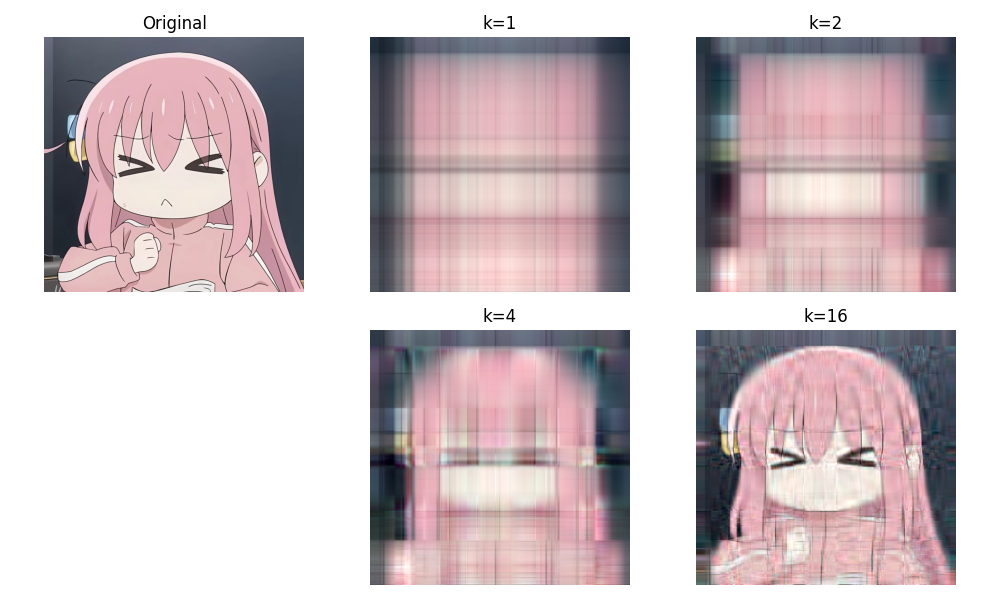
\includegraphics[width=0.8\linewidth]{figures/SVD.png}
    \caption{Reconstruction Results}
\end{figure}

When $k$ grows larger, the quality is better. In the code, I calculate Frobenius norm with np.linalg.norm, and it's equivalent with using the square sum of singular values. In this photo, the percentage of Frobenius norm is:
\begin{itemize}[noitemsep]
    \item $k = 1$: $96.21\%$
    \item $k = 2$: $96.90\%$
    \item $k = 4$: $97.51\%$
    \item $k = 16$: $98.59\%$
\end{itemize}
    
\end{answer}

\end{document}